% Options for packages loaded elsewhere
\PassOptionsToPackage{unicode}{hyperref}
\PassOptionsToPackage{hyphens}{url}
%
\documentclass[
]{article}
\title{S2. Additional figures and table}
\author{}
\date{\vspace{-2.5em}2022-02-19}

\usepackage{amsmath,amssymb}
\usepackage{lmodern}
\usepackage{iftex}
\ifPDFTeX
  \usepackage[T1]{fontenc}
  \usepackage[utf8]{inputenc}
  \usepackage{textcomp} % provide euro and other symbols
\else % if luatex or xetex
  \usepackage{unicode-math}
  \defaultfontfeatures{Scale=MatchLowercase}
  \defaultfontfeatures[\rmfamily]{Ligatures=TeX,Scale=1}
\fi
% Use upquote if available, for straight quotes in verbatim environments
\IfFileExists{upquote.sty}{\usepackage{upquote}}{}
\IfFileExists{microtype.sty}{% use microtype if available
  \usepackage[]{microtype}
  \UseMicrotypeSet[protrusion]{basicmath} % disable protrusion for tt fonts
}{}
\makeatletter
\@ifundefined{KOMAClassName}{% if non-KOMA class
  \IfFileExists{parskip.sty}{%
    \usepackage{parskip}
  }{% else
    \setlength{\parindent}{0pt}
    \setlength{\parskip}{6pt plus 2pt minus 1pt}}
}{% if KOMA class
  \KOMAoptions{parskip=half}}
\makeatother
\usepackage{xcolor}
\IfFileExists{xurl.sty}{\usepackage{xurl}}{} % add URL line breaks if available
\IfFileExists{bookmark.sty}{\usepackage{bookmark}}{\usepackage{hyperref}}
\hypersetup{
  pdftitle={S2. Additional figures and table},
  hidelinks,
  pdfcreator={LaTeX via pandoc}}
\urlstyle{same} % disable monospaced font for URLs
\usepackage[margin=1in]{geometry}
\usepackage{graphicx}
\makeatletter
\def\maxwidth{\ifdim\Gin@nat@width>\linewidth\linewidth\else\Gin@nat@width\fi}
\def\maxheight{\ifdim\Gin@nat@height>\textheight\textheight\else\Gin@nat@height\fi}
\makeatother
% Scale images if necessary, so that they will not overflow the page
% margins by default, and it is still possible to overwrite the defaults
% using explicit options in \includegraphics[width, height, ...]{}
\setkeys{Gin}{width=\maxwidth,height=\maxheight,keepaspectratio}
% Set default figure placement to htbp
\makeatletter
\def\fps@figure{htbp}
\makeatother
\setlength{\emergencystretch}{3em} % prevent overfull lines
\providecommand{\tightlist}{%
  \setlength{\itemsep}{0pt}\setlength{\parskip}{0pt}}
\setcounter{secnumdepth}{-\maxdimen} % remove section numbering
\usepackage{caption}
\usepackage{placeins}
\usepackage{amsmath}
\usepackage{lineno}
\linenumbers
\captionsetup[table]{labelformat=empty}
\captionsetup[figure]{labelformat=empty}
\usepackage{booktabs}
\usepackage{longtable}
\usepackage{array}
\usepackage{multirow}
\usepackage{wrapfig}
\usepackage{float}
\usepackage{colortbl}
\usepackage{pdflscape}
\usepackage{tabu}
\usepackage{threeparttable}
\usepackage{threeparttablex}
\usepackage[normalem]{ulem}
\usepackage{makecell}
\usepackage{xcolor}
\ifLuaTeX
  \usepackage{selnolig}  % disable illegal ligatures
\fi

\begin{document}
\maketitle

{
\setcounter{tocdepth}{2}
\tableofcontents
}
\newpage

\hypertarget{posterior-predictive-distributions}{%
\section{Posterior predictive
distributions}\label{posterior-predictive-distributions}}

Figure 1 show the mixture of the PPD of the probability of a positive
match, grouped by label (only records manually labelled or reviewed are
considered). The posterior samples for each record were extracted and
joined into a global distribution; on this distribution, density was
computed on the logit scale and then logistic transformed for displaying
on a \([0 - 1]\) scale. The purple ridges show the distribution of the
still unlabelled records.\\
For each iteration, the thresholds which define the ``uncertainty
zone'', i.e, the lower and the upper range of 98\% PrI for the positive
and negative records respectively, are shown. Records whose 98\% PrI
intersects the uncertainty zone requires manual review.\\
Notice how the positive and negative record densities tend to
increasingly overlap at each iteration; meanwhile the distribution of
the records to be reviewed shrinks and shifts towards the negative side,
as positive records get found and labeled.\\
In Session 2, as the number of negative records reviewed increased, also
already positively labelled records re-entered the uncertainty zone;
this is due to the baseline positivity rate decreasing as the number of
negatives in the training data increased, forcing to review dubious
records that may have been mislabelled.

\begin{figure}
\centering
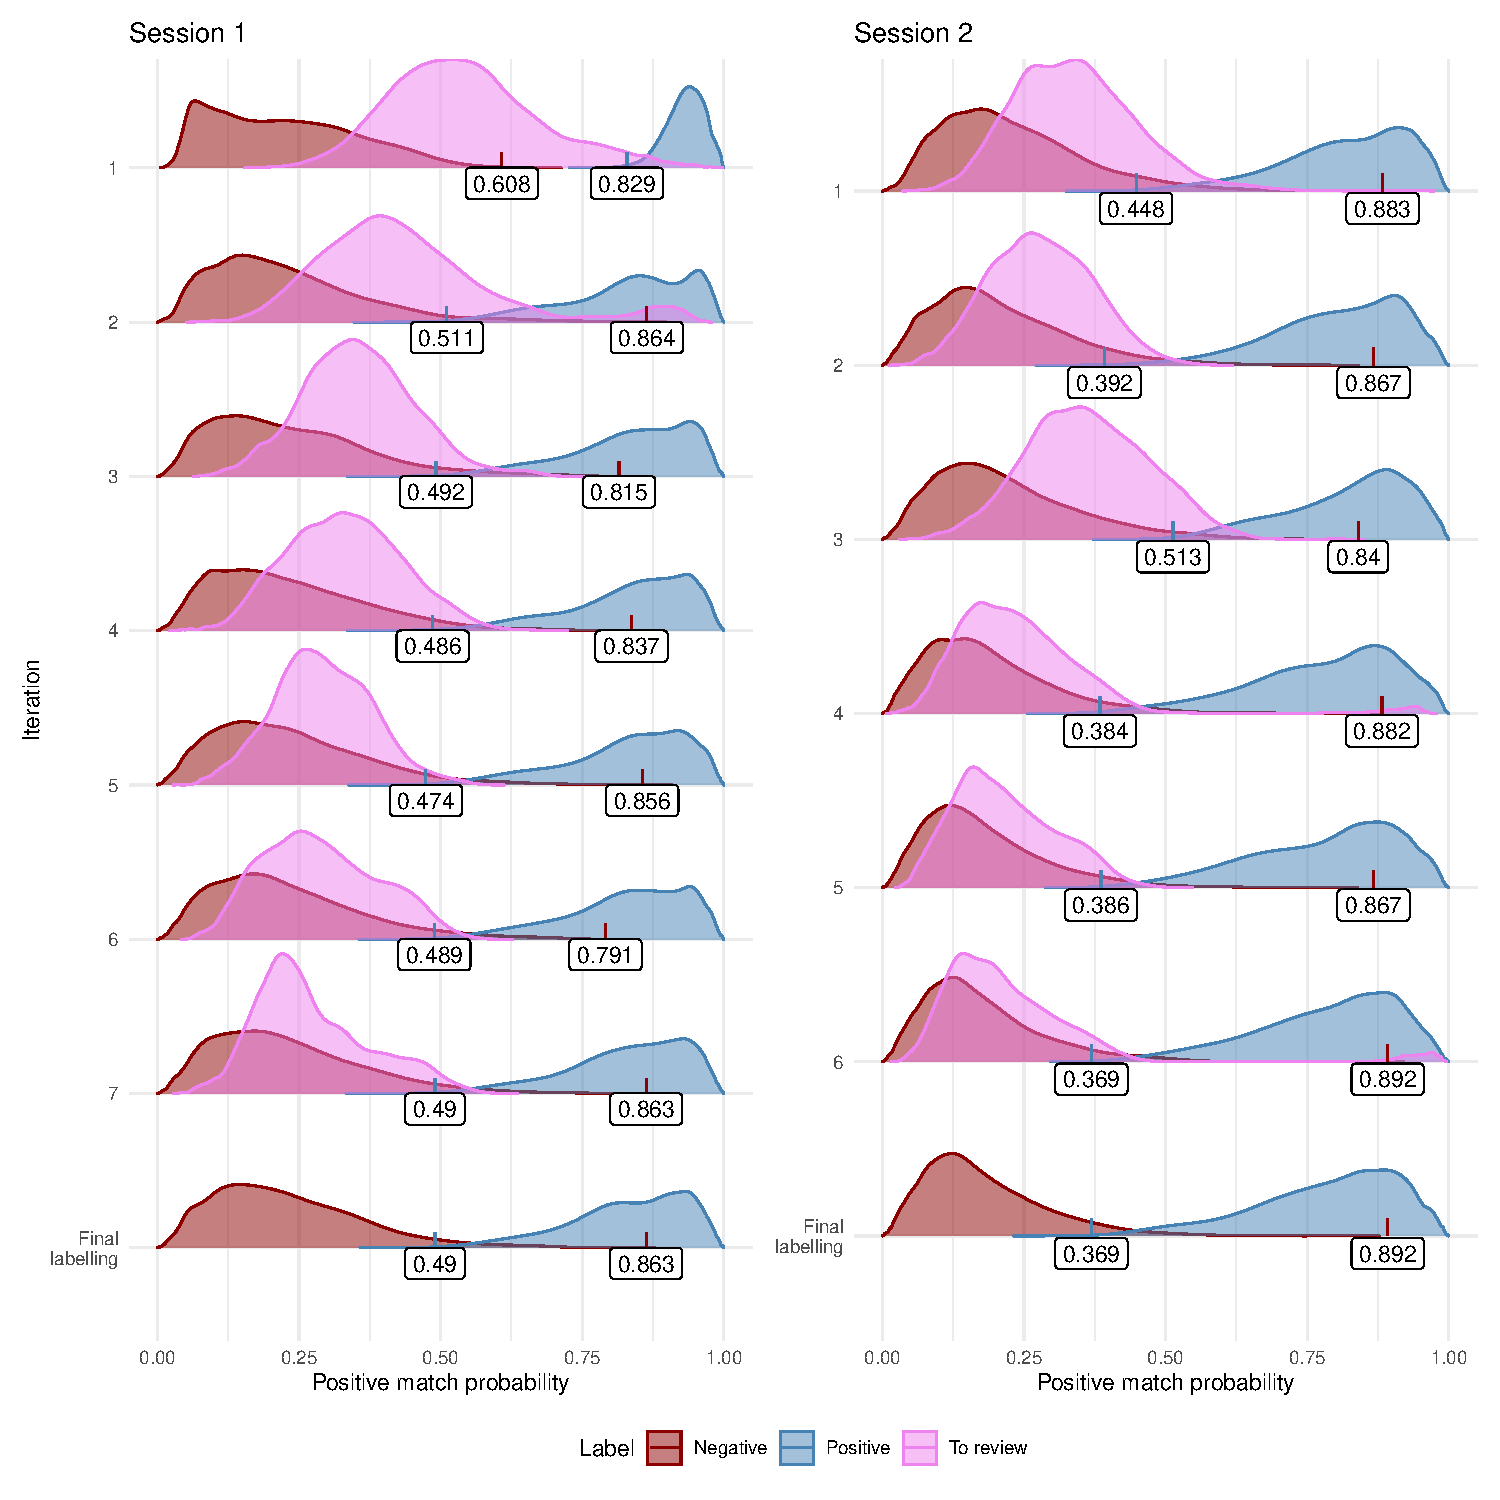
\includegraphics{S2.Additional_outputs_files/figure-latex/posterior_distributions-1.pdf}
\caption{\textbf{Figure 1}. Mixture predictive distribution of the
probability of a positive match, grouped by labelling status.}
\end{figure}

\hypertarget{list-of-terms-relevant-for-prediction}{%
\section{List of terms relevant for
prediction}\label{list-of-terms-relevant-for-prediction}}

In table 1 and 2 are listed the 50 more relevant terms used by the BART
algorithm to discriminate between positive and negative records, for
Session 1 and 2 (see Methods). Term importance (``Inclusion rate'' in
the tables) is defined as the ensemble average inclusion rate in
posterior trees over 10,000 total term inclusions, while the Inclusion
Stability (IS) is the ratio of the average inclusion rate over its
standard deviation among the ensemble models. The symbol ``\textbar{}''
in the terms indicate redundant terms while ``\&'' indicate nc-grams.
The component in which the term was used is reported in the leftmost
column.\\
For each term, we added its linear association with a positive label
estimated through a Poisson regression, reporting it as Relative Risk
(RR) and its statistical significance (Statistic) measured as number of
standard errors, s.e., of the terms. A strong BART score with a
Statistic close to zero identify terms whose effect is highly non-linear
(e.g., they are relevant only in the presence of other terms).

\begin{table}[!h]

\caption{\label{tab:var imp}\textbf{Table 1}. Term importance at the end of Session 1.}
\centering
\resizebox{\linewidth}{!}{
\begin{tabular}[t]{llllll}
\toprule
Component & Term & Inclusion rate & IS & RR & Statistic\\
\midrule
\cellcolor{gray!6}{Keyword} & \cellcolor{gray!6}{Patient Transport} & \cellcolor{gray!6}{61.2} & \cellcolor{gray!6}{3.77} & \cellcolor{gray!6}{99.1} & \cellcolor{gray!6}{21.3}\\
Abstract & Transfer & 57 & 3.93 & 22.5 & 15.4\\
\cellcolor{gray!6}{Title} & \cellcolor{gray!6}{Network} & \cellcolor{gray!6}{56.5} & \cellcolor{gray!6}{2.91} & \cellcolor{gray!6}{18} & \cellcolor{gray!6}{14.2}\\
Abstract & Network \& Patient & 54.2 & 4.66 & 26.3 & 15.2\\
\cellcolor{gray!6}{Author} & \cellcolor{gray!6}{Donker T} & \cellcolor{gray!6}{53.5} & \cellcolor{gray!6}{4.56} & \cellcolor{gray!6}{159} & \cellcolor{gray!6}{16.5}\\
\addlinespace
Abstract & Worker & 50 & 3.33 & 0.421 & -1.21\\
\cellcolor{gray!6}{Keyword} & \cellcolor{gray!6}{Hospitals} & \cellcolor{gray!6}{49.8} & \cellcolor{gray!6}{4.31} & \cellcolor{gray!6}{27.8} & \cellcolor{gray!6}{16.5}\\
Abstract & Movement & 47.8 & 2.7 & 27.2 & 15\\
\cellcolor{gray!6}{Title} & \cellcolor{gray!6}{Spread} & \cellcolor{gray!6}{46.6} & \cellcolor{gray!6}{2.25} & \cellcolor{gray!6}{16.2} & \cellcolor{gray!6}{12.1}\\
Abstract & Facility & 45 & 2.22 & 19.6 & 14.8\\
\addlinespace
\cellcolor{gray!6}{Keyword} & \cellcolor{gray!6}{Orange County} & \cellcolor{gray!6}{44.3} & \cellcolor{gray!6}{3.19} & \cellcolor{gray!6}{199} & \cellcolor{gray!6}{17.2}\\
Abstract & Conduct & 42.6 & 3.7 & 0.221 & -2.57\\
\cellcolor{gray!6}{Abstract} & \cellcolor{gray!6}{Patient} & \cellcolor{gray!6}{42} & \cellcolor{gray!6}{3.61} & \cellcolor{gray!6}{27.6} & \cellcolor{gray!6}{7.23}\\
Abstract & Perform & 41.9 & 2.38 & 0.342 & -2.55\\
\cellcolor{gray!6}{Title} & \cellcolor{gray!6}{Hospital} & \cellcolor{gray!6}{39} & \cellcolor{gray!6}{1.95} & \cellcolor{gray!6}{12.5} & \cellcolor{gray!6}{12.5}\\
\addlinespace
Abstract & Regional & 38.9 & 3.08 & 21.7 & 14.9\\
\cellcolor{gray!6}{Abstract} & \cellcolor{gray!6}{Agent} & \cellcolor{gray!6}{38.1} & \cellcolor{gray!6}{2.74} & \cellcolor{gray!6}{4.36} & \cellcolor{gray!6}{6.28}\\
Abstract & California & 37.3 & 2.6 & 38 & 12.6\\
\cellcolor{gray!6}{Title} & \cellcolor{gray!6}{Transfer} & \cellcolor{gray!6}{36.6} & \cellcolor{gray!6}{3.54} & \cellcolor{gray!6}{27} & \cellcolor{gray!6}{11.8}\\
Keyword & Patient Transfer | Patient Transfer \& Patient Transport & 36.6 & 2.16 & 164 & 2\\
\addlinespace
\cellcolor{gray!6}{Abstract} & \cellcolor{gray!6}{Finding} & \cellcolor{gray!6}{33.2} & \cellcolor{gray!6}{1.78} & \cellcolor{gray!6}{0.372} & \cellcolor{gray!6}{-2.35}\\
Title & Outbreak & 32.9 & 2.91 & 3.4 & 3.51\\
\cellcolor{gray!6}{Abstract} & \cellcolor{gray!6}{Collect} & \cellcolor{gray!6}{32.4} & \cellcolor{gray!6}{1.82} & \cellcolor{gray!6}{0.408} & \cellcolor{gray!6}{-1.95}\\
Title & Regional & 32.3 & 2.68 & 44.2 & 14.2\\
\cellcolor{gray!6}{Abstract} & \cellcolor{gray!6}{Network} & \cellcolor{gray!6}{31.6} & \cellcolor{gray!6}{3.09} & \cellcolor{gray!6}{12.8} & \cellcolor{gray!6}{11.7}\\
\addlinespace
Abstract & Resistant & 31.6 & 2.55 & 11 & 11.2\\
\cellcolor{gray!6}{Abstract} & \cellcolor{gray!6}{Outcome} & \cellcolor{gray!6}{31.2} & \cellcolor{gray!6}{1.93} & \cellcolor{gray!6}{0.178} & \cellcolor{gray!6}{-2.95}\\
Abstract & Discharge & 31.1 & 3.79 & 9.99 & 9.02\\
\cellcolor{gray!6}{Abstract} & \cellcolor{gray!6}{2014} & \cellcolor{gray!6}{30.3} & \cellcolor{gray!6}{1.84} & \cellcolor{gray!6}{0.588} & \cellcolor{gray!6}{-1.04}\\
Abstract & Practice & 29.5 & 2.47 & 0.508 & -1.33\\
\addlinespace
\cellcolor{gray!6}{Abstract} & \cellcolor{gray!6}{Culture} & \cellcolor{gray!6}{28.9} & \cellcolor{gray!6}{2.14} & \cellcolor{gray!6}{0.378} & \cellcolor{gray!6}{-1.66}\\
Abstract & Positive & 28.8 & 1.96 & 0.346 & -2.52\\
\cellcolor{gray!6}{Abstract} & \cellcolor{gray!6}{Gene} & \cellcolor{gray!6}{28.3} & \cellcolor{gray!6}{1.29} & \cellcolor{gray!6}{0.00000024} & \cellcolor{gray!6}{-0.0415}\\
Abstract & Disease & 28 & 2.42 & 0.365 & -3.7\\
\cellcolor{gray!6}{Keyword} & \cellcolor{gray!6}{Enterococci} & \cellcolor{gray!6}{27.5} & \cellcolor{gray!6}{1.92} & \cellcolor{gray!6}{25.2} & \cellcolor{gray!6}{6.33}\\
\addlinespace
Abstract & Month & 27.3 & 1.86 & 0.288 & -2.44\\
\cellcolor{gray!6}{Abstract} & \cellcolor{gray!6}{Healthcare \& Facility} & \cellcolor{gray!6}{26.2} & \cellcolor{gray!6}{1.74} & \cellcolor{gray!6}{34.9} & \cellcolor{gray!6}{17}\\
Abstract & Prevalence & 26.2 & 1.71 & 4.08 & 6.69\\
\cellcolor{gray!6}{Abstract} & \cellcolor{gray!6}{Effort} & \cellcolor{gray!6}{26.1} & \cellcolor{gray!6}{1.22} & \cellcolor{gray!6}{6.64} & \cellcolor{gray!6}{8.57}\\
Abstract & Length & 25.3 & 1.44 & 6.1 & 6.45\\
\addlinespace
\cellcolor{gray!6}{Keyword} & \cellcolor{gray!6}{System} & \cellcolor{gray!6}{25} & \cellcolor{gray!6}{1.43} & \cellcolor{gray!6}{11.9} & \cellcolor{gray!6}{3.47}\\
Abstract & Laboratory & 24.4 & 1.38 & 0.442 & -1.39\\
\cellcolor{gray!6}{Keyword} & \cellcolor{gray!6}{Resistant Staphylococcus Aureus} & \cellcolor{gray!6}{24.4} & \cellcolor{gray!6}{1.59} & \cellcolor{gray!6}{22.8} & \cellcolor{gray!6}{11.2}\\
Abstract & Clinical & 23.6 & 2.1 & 0.421 & -2.9\\
\cellcolor{gray!6}{Abstract} & \cellcolor{gray!6}{Dataset} & \cellcolor{gray!6}{22.5} & \cellcolor{gray!6}{1.47} & \cellcolor{gray!6}{8.75} & \cellcolor{gray!6}{6.5}\\
\addlinespace
Abstract & Development & 22.2 & 1.22 & 0.148 & -2.68\\
\cellcolor{gray!6}{Abstract} & \cellcolor{gray!6}{Hand} & \cellcolor{gray!6}{22} & \cellcolor{gray!6}{1.97} & \cellcolor{gray!6}{0.822} & \cellcolor{gray!6}{-0.335}\\
Keyword & Pathogen Transmission & 21.8 & 3.26 & 67.9 & 7.2\\
\cellcolor{gray!6}{Keyword} & \cellcolor{gray!6}{Cross Infection \& Humans \& Transmission} & \cellcolor{gray!6}{21.7} & \cellcolor{gray!6}{1.4} & \cellcolor{gray!6}{31.1} & \cellcolor{gray!6}{15.5}\\
Abstract & Flow & 21.4 & 1.14 & 4.07 & 4.56\\
\bottomrule
\end{tabular}}
\end{table}

\begin{table}[!h]

\caption{\label{tab:var imp}\textbf{Table 2}. Term importance at the end of Session 2.}
\centering
\resizebox{\linewidth}{!}{
\begin{tabular}[t]{llllll}
\toprule
Component & Term & Inclusion rate & IS & RR & Statistic\\
\midrule
\cellcolor{gray!6}{Keyword} & \cellcolor{gray!6}{Patient Transport} & \cellcolor{gray!6}{61.2} & \cellcolor{gray!6}{3.77} & \cellcolor{gray!6}{99.1} & \cellcolor{gray!6}{21.3}\\
Abstract & Transfer & 57 & 3.93 & 22.5 & 15.4\\
\cellcolor{gray!6}{Title} & \cellcolor{gray!6}{Network} & \cellcolor{gray!6}{56.5} & \cellcolor{gray!6}{2.91} & \cellcolor{gray!6}{18} & \cellcolor{gray!6}{14.2}\\
Abstract & Network \& Patient & 54.2 & 4.66 & 26.3 & 15.2\\
\cellcolor{gray!6}{Author} & \cellcolor{gray!6}{Donker T} & \cellcolor{gray!6}{53.5} & \cellcolor{gray!6}{4.56} & \cellcolor{gray!6}{159} & \cellcolor{gray!6}{16.5}\\
\addlinespace
Abstract & Worker & 50 & 3.33 & 0.421 & -1.21\\
\cellcolor{gray!6}{Keyword} & \cellcolor{gray!6}{Hospitals} & \cellcolor{gray!6}{49.8} & \cellcolor{gray!6}{4.31} & \cellcolor{gray!6}{27.8} & \cellcolor{gray!6}{16.5}\\
Abstract & Movement & 47.8 & 2.7 & 27.2 & 15\\
\cellcolor{gray!6}{Title} & \cellcolor{gray!6}{Spread} & \cellcolor{gray!6}{46.6} & \cellcolor{gray!6}{2.25} & \cellcolor{gray!6}{16.2} & \cellcolor{gray!6}{12.1}\\
Abstract & Facility & 45 & 2.22 & 19.6 & 14.8\\
\addlinespace
\cellcolor{gray!6}{Keyword} & \cellcolor{gray!6}{Orange County} & \cellcolor{gray!6}{44.3} & \cellcolor{gray!6}{3.19} & \cellcolor{gray!6}{199} & \cellcolor{gray!6}{17.2}\\
Abstract & Conduct & 42.6 & 3.7 & 0.221 & -2.57\\
\cellcolor{gray!6}{Abstract} & \cellcolor{gray!6}{Patient} & \cellcolor{gray!6}{42} & \cellcolor{gray!6}{3.61} & \cellcolor{gray!6}{27.6} & \cellcolor{gray!6}{7.23}\\
Abstract & Perform & 41.9 & 2.38 & 0.342 & -2.55\\
\cellcolor{gray!6}{Title} & \cellcolor{gray!6}{Hospital} & \cellcolor{gray!6}{39} & \cellcolor{gray!6}{1.95} & \cellcolor{gray!6}{12.5} & \cellcolor{gray!6}{12.5}\\
\addlinespace
Abstract & Regional & 38.9 & 3.08 & 21.7 & 14.9\\
\cellcolor{gray!6}{Abstract} & \cellcolor{gray!6}{Agent} & \cellcolor{gray!6}{38.1} & \cellcolor{gray!6}{2.74} & \cellcolor{gray!6}{4.36} & \cellcolor{gray!6}{6.28}\\
Abstract & California & 37.3 & 2.6 & 38 & 12.6\\
\cellcolor{gray!6}{Title} & \cellcolor{gray!6}{Transfer} & \cellcolor{gray!6}{36.6} & \cellcolor{gray!6}{3.54} & \cellcolor{gray!6}{27} & \cellcolor{gray!6}{11.8}\\
Keyword & Patient Transfer | Patient Transfer \& Patient Transport & 36.6 & 2.16 & 164 & 2\\
\addlinespace
\cellcolor{gray!6}{Abstract} & \cellcolor{gray!6}{Finding} & \cellcolor{gray!6}{33.2} & \cellcolor{gray!6}{1.78} & \cellcolor{gray!6}{0.372} & \cellcolor{gray!6}{-2.35}\\
Title & Outbreak & 32.9 & 2.91 & 3.4 & 3.51\\
\cellcolor{gray!6}{Abstract} & \cellcolor{gray!6}{Collect} & \cellcolor{gray!6}{32.4} & \cellcolor{gray!6}{1.82} & \cellcolor{gray!6}{0.408} & \cellcolor{gray!6}{-1.95}\\
Title & Regional & 32.3 & 2.68 & 44.2 & 14.2\\
\cellcolor{gray!6}{Abstract} & \cellcolor{gray!6}{Network} & \cellcolor{gray!6}{31.6} & \cellcolor{gray!6}{3.09} & \cellcolor{gray!6}{12.8} & \cellcolor{gray!6}{11.7}\\
\addlinespace
Abstract & Resistant & 31.6 & 2.55 & 11 & 11.2\\
\cellcolor{gray!6}{Abstract} & \cellcolor{gray!6}{Outcome} & \cellcolor{gray!6}{31.2} & \cellcolor{gray!6}{1.93} & \cellcolor{gray!6}{0.178} & \cellcolor{gray!6}{-2.95}\\
Abstract & Discharge & 31.1 & 3.79 & 9.99 & 9.02\\
\cellcolor{gray!6}{Abstract} & \cellcolor{gray!6}{2014} & \cellcolor{gray!6}{30.3} & \cellcolor{gray!6}{1.84} & \cellcolor{gray!6}{0.588} & \cellcolor{gray!6}{-1.04}\\
Abstract & Practice & 29.5 & 2.47 & 0.508 & -1.33\\
\addlinespace
\cellcolor{gray!6}{Abstract} & \cellcolor{gray!6}{Culture} & \cellcolor{gray!6}{28.9} & \cellcolor{gray!6}{2.14} & \cellcolor{gray!6}{0.378} & \cellcolor{gray!6}{-1.66}\\
Abstract & Positive & 28.8 & 1.96 & 0.346 & -2.52\\
\cellcolor{gray!6}{Abstract} & \cellcolor{gray!6}{Gene} & \cellcolor{gray!6}{28.3} & \cellcolor{gray!6}{1.29} & \cellcolor{gray!6}{0.00000024} & \cellcolor{gray!6}{-0.0415}\\
Abstract & Disease & 28 & 2.42 & 0.365 & -3.7\\
\cellcolor{gray!6}{Keyword} & \cellcolor{gray!6}{Enterococci} & \cellcolor{gray!6}{27.5} & \cellcolor{gray!6}{1.92} & \cellcolor{gray!6}{25.2} & \cellcolor{gray!6}{6.33}\\
\addlinespace
Abstract & Month & 27.3 & 1.86 & 0.288 & -2.44\\
\cellcolor{gray!6}{Abstract} & \cellcolor{gray!6}{Healthcare \& Facility} & \cellcolor{gray!6}{26.2} & \cellcolor{gray!6}{1.74} & \cellcolor{gray!6}{34.9} & \cellcolor{gray!6}{17}\\
Abstract & Prevalence & 26.2 & 1.71 & 4.08 & 6.69\\
\cellcolor{gray!6}{Abstract} & \cellcolor{gray!6}{Effort} & \cellcolor{gray!6}{26.1} & \cellcolor{gray!6}{1.22} & \cellcolor{gray!6}{6.64} & \cellcolor{gray!6}{8.57}\\
Abstract & Length & 25.3 & 1.44 & 6.1 & 6.45\\
\addlinespace
\cellcolor{gray!6}{Keyword} & \cellcolor{gray!6}{System} & \cellcolor{gray!6}{25} & \cellcolor{gray!6}{1.43} & \cellcolor{gray!6}{11.9} & \cellcolor{gray!6}{3.47}\\
Abstract & Laboratory & 24.4 & 1.38 & 0.442 & -1.39\\
\cellcolor{gray!6}{Keyword} & \cellcolor{gray!6}{Resistant Staphylococcus Aureus} & \cellcolor{gray!6}{24.4} & \cellcolor{gray!6}{1.59} & \cellcolor{gray!6}{22.8} & \cellcolor{gray!6}{11.2}\\
Abstract & Clinical & 23.6 & 2.1 & 0.421 & -2.9\\
\cellcolor{gray!6}{Abstract} & \cellcolor{gray!6}{Dataset} & \cellcolor{gray!6}{22.5} & \cellcolor{gray!6}{1.47} & \cellcolor{gray!6}{8.75} & \cellcolor{gray!6}{6.5}\\
\addlinespace
Abstract & Development & 22.2 & 1.22 & 0.148 & -2.68\\
\cellcolor{gray!6}{Abstract} & \cellcolor{gray!6}{Hand} & \cellcolor{gray!6}{22} & \cellcolor{gray!6}{1.97} & \cellcolor{gray!6}{0.822} & \cellcolor{gray!6}{-0.335}\\
Keyword & Pathogen Transmission & 21.8 & 3.26 & 67.9 & 7.2\\
\cellcolor{gray!6}{Keyword} & \cellcolor{gray!6}{Cross Infection \& Humans \& Transmission} & \cellcolor{gray!6}{21.7} & \cellcolor{gray!6}{1.4} & \cellcolor{gray!6}{31.1} & \cellcolor{gray!6}{15.5}\\
Abstract & Flow & 21.4 & 1.14 & 4.07 & 4.56\\
\bottomrule
\end{tabular}}
\end{table}

\hypertarget{hyperparameters-grid-search}{%
\section{Hyperparameters grid
search}\label{hyperparameters-grid-search}}

Table 3 shows the best hyperparameter set and their performance for each
cluster while figure 2 displays the conditional impact on performance of
each hyperparameter.

The most influential parameters were the number of models in the
ensemble, the oversampling rate and the initial training set size. The
use of bootstrap resampling seemed detrimental.

\begin{figure}
\centering
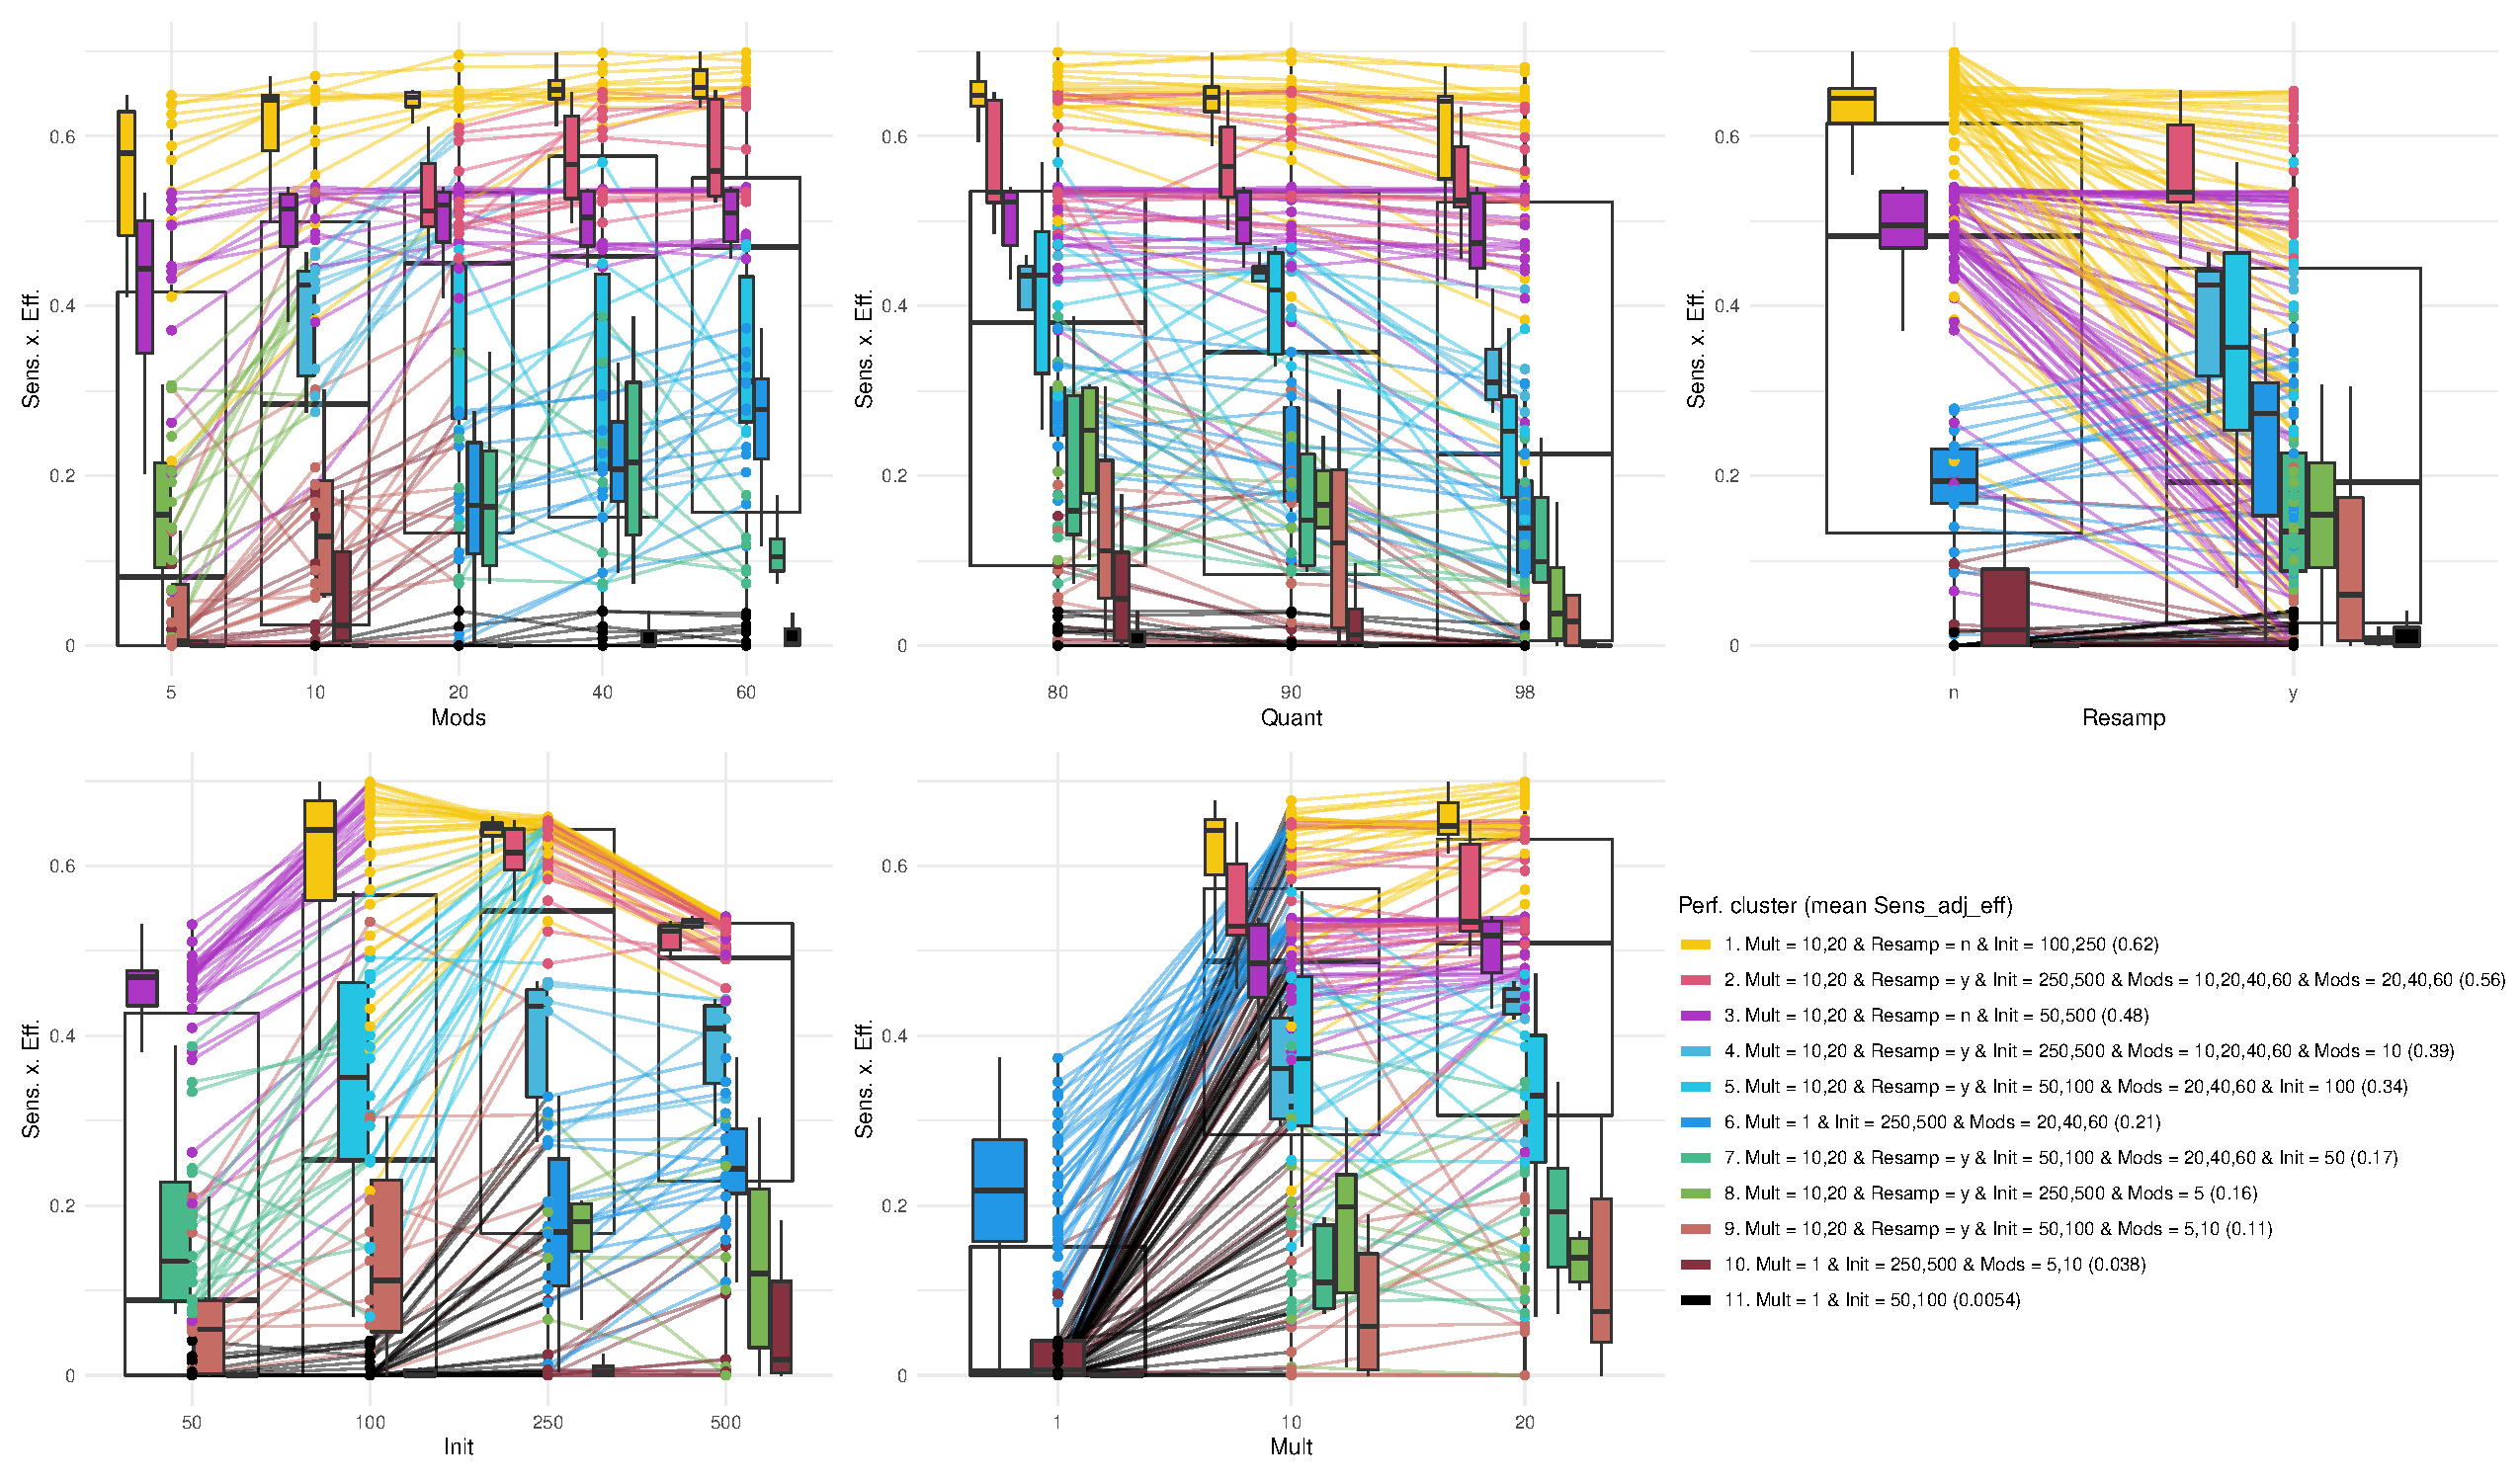
\includegraphics{S2.Additional_outputs_files/figure-latex/hyperparameters-1.pdf}
\caption{\textbf{Figure 2}. Score clusters and impact of single
hyperparameters on engine performance. The performance is measured as
Sensitivity x Efficiency. Each cluster is color coded. Mods: number of
models in the ensemble; Quant: PrI quantiles for the uncertainty zone;
Resamp: bootstrap resampling between models; Init: size of initial
training set; Multi: oversampling rate of positive records}
\end{figure}

\begin{table}[!h]

\caption{\label{tab:hyperparameters}\textbf{Table 3}. Hyperparameter clusters and best cluster subsets. For each cluster, the defining rules and mean Sens. x Eff. is shown, followed by the per-cluster best set results.}
\centering
\resizebox{\linewidth}{!}{
\begin{tabular}[t]{llllllllllll}
\toprule
Cluster (mean score) & Num. iterations & Positive matches & Reviewed records & Sensitivity & Efficiency & Score (Sens. x Eff.) & Num. ensemble models & Uncertainty interval & Resampling & Num. initial training records & Positives oversampling multiplier\\
\midrule
\cellcolor{gray!6}{1. Mult = 10,20 \& Mods = 10,20,40,60 \& Resamp = n \& Init = 100,250 (0.64)} & \cellcolor{gray!6}{7} & \cellcolor{gray!6}{81 / 82} & \cellcolor{gray!6}{462 / 1200} & \cellcolor{gray!6}{98.8\%} & \cellcolor{gray!6}{61.5\%} & \cellcolor{gray!6}{0.608} & \cellcolor{gray!6}{10} & \cellcolor{gray!6}{98} & \cellcolor{gray!6}{n} & \cellcolor{gray!6}{250} & \cellcolor{gray!6}{10}\\
2. Mult = 10,20 \& Mods = 10,20,40,60 \& Resamp = y \& Init = 250,500 \& Mods = 20,40,60 (0.56) & 5 & 82 / 82 & 618 / 1200 & 100\% & 48.5\% & 0.485 & 20 & 80 & y & 250 & 10\\
\cellcolor{gray!6}{3. Mult = 10,20 \& Mods = 10,20,40,60 \& Resamp = n \& Init = 50,500 (0.5)} & \cellcolor{gray!6}{6} & \cellcolor{gray!6}{81 / 82} & \cellcolor{gray!6}{589 / 1200} & \cellcolor{gray!6}{98.8\%} & \cellcolor{gray!6}{50.9\%} & \cellcolor{gray!6}{0.503} & \cellcolor{gray!6}{10} & \cellcolor{gray!6}{98} & \cellcolor{gray!6}{n} & \cellcolor{gray!6}{500} & \cellcolor{gray!6}{10}\\
4. Mult = 10,20 \& Mods = 1,5 \& Resamp = n \& Mods = 5 (0.47) & 8 & 82 / 82 & 1123 / 1200 & 100\% & 6.42\% & 0.0642 & 5 & 98 & n & 50 & 10\\
\cellcolor{gray!6}{5. Mult = 10,20 \& Mods = 10,20,40,60 \& Resamp = y \& Init = 250,500 \& Mods = 10 (0.39)} & \cellcolor{gray!6}{5} & \cellcolor{gray!6}{82 / 82} & \cellcolor{gray!6}{685 / 1200} & \cellcolor{gray!6}{100\%} & \cellcolor{gray!6}{42.9\%} & \cellcolor{gray!6}{0.429} & \cellcolor{gray!6}{10} & \cellcolor{gray!6}{80} & \cellcolor{gray!6}{y} & \cellcolor{gray!6}{250} & \cellcolor{gray!6}{10}\\
\addlinespace
6. Mult = 10,20 \& Mods = 1,5 \& Resamp = n \& Mods = 1 \& Init = 250,500 (0.31) & 5 & 82 / 82 & 874 / 1200 & 100\% & 27.2\% & 0.272 & 1 & 90 & n & 250 & 10\\
\cellcolor{gray!6}{7. Mult = 10,20 \& Mods = 10,20,40,60 \& Resamp = y \& Init = 50,100 (0.23)} & \cellcolor{gray!6}{7} & \cellcolor{gray!6}{82 / 82} & \cellcolor{gray!6}{948 / 1200} & \cellcolor{gray!6}{100\%} & \cellcolor{gray!6}{21\%} & \cellcolor{gray!6}{0.21} & \cellcolor{gray!6}{10} & \cellcolor{gray!6}{90} & \cellcolor{gray!6}{y} & \cellcolor{gray!6}{50} & \cellcolor{gray!6}{20}\\
8. Mult = 1 \& Init = 250,500 \& Mods = 20,40,60 (0.21) & 5 & 82 / 82 & 806 / 1200 & 100\% & 32.8\% & 0.328 & 60 & 80 & y & 250 & 1\\
\cellcolor{gray!6}{9. Mult = 10,20 \& Mods = 1,5 \& Resamp = n \& Mods = 1 \& Init = 50,100 (0.078)} & \cellcolor{gray!6}{6} & \cellcolor{gray!6}{82 / 82} & \cellcolor{gray!6}{1139 / 1200} & \cellcolor{gray!6}{100\%} & \cellcolor{gray!6}{5.08\%} & \cellcolor{gray!6}{0.0508} & \cellcolor{gray!6}{1} & \cellcolor{gray!6}{90} & \cellcolor{gray!6}{n} & \cellcolor{gray!6}{50} & \cellcolor{gray!6}{20}\\
10. Mult = 10,20 \& Mods = 1,5 \& Resamp = y (0.054) & 5 & 82 / 82 & 832 / 1200 & 100\% & 30.7\% & 0.307 & 5 & 80 & y & 250 & 20\\
\addlinespace
\cellcolor{gray!6}{11. Mult = 1 \& Init = 250,500 \& Mods = 1,5,10 (0.025)} & \cellcolor{gray!6}{5} & \cellcolor{gray!6}{82 / 82} & \cellcolor{gray!6}{981 / 1200} & \cellcolor{gray!6}{100\%} & \cellcolor{gray!6}{18.2\%} & \cellcolor{gray!6}{0.182} & \cellcolor{gray!6}{10} & \cellcolor{gray!6}{90} & \cellcolor{gray!6}{y} & \cellcolor{gray!6}{500} & \cellcolor{gray!6}{1}\\
12. Mult = 1 \& Init = 50,100 (0.0045) & 6 & 82 / 82 & 1151 / 1200 & 100\% & 4.08\% & 0.0408 & 20 & 80 & y & 50 & 1\\
\bottomrule
\end{tabular}}
\end{table}

\end{document}
